\documentclass[11pt]{article}
\usepackage{fontspec}
\usepackage[spanish]{babel}
\usepackage[utf8]{inputenc}

%Tipo de letra y color
\usepackage{FiraSans}        % Fuente sans serif
\usepackage[usenames]{color}
\definecolor{ColorTitulo}{RGB}{169,50,38}

%Imágenes
\usepackage{graphicx}
\graphicspath{{img/}}
\usepackage{float}

%Matemáticas
\usepackage{amssymb}
\usepackage{amsmath}

%Código
\usepackage{listings}
%\usepackage{xcolor}
\renewcommand{\lstlistingname}{Código}% Listing -> Código

\definecolor{dkgreen}{rgb}{0,0.6,0}
\definecolor{gray}{rgb}{0.5,0.5,0.5}
\definecolor{mauve}{rgb}{0.58,0,0.82}
\definecolor{codegreen}{rgb}{0,0.6,0}
\definecolor{codegray}{rgb}{0.5,0.5,0.5}
\definecolor{codepurple}{rgb}{0.58,0,0.82}
\definecolor{backcolour}{rgb}{0.95,0.95,0.92}
\definecolor{titlecolour}{rgb}{0.05, 0.63,0.41}
 
\lstdefinestyle{mystyle}{
    backgroundcolor=\color{backcolour},   
    commentstyle=\color{titlecolour},
    keywordstyle=\color{ColorTitulo},
    numberstyle=\tiny\color{codegray},
    stringstyle=\color{ColorTitulo},
    basicstyle=\ttfamily\footnotesize,
    breakatwhitespace=false,         
    breaklines=true,                 
    captionpos=b,                    
    keepspaces=true,                 
    numbers=left,                    
    numbersep=5pt,                  
    showspaces=false,                
    showstringspaces=false,
    showtabs=false,                  
    tabsize=2
}
\lstset{style=mystyle}

%Márgenes
\usepackage[paper=portrait, pagesize]{typearea}
\usepackage{titlepic}
\setlength{\textwidth}{155mm}
\setlength{\textheight}{210mm}
\setlength{\oddsidemargin}{6mm}
\setlength{\evensidemargin}{28mm}
\setlength{\topmargin}{-10mm}
\setlength\parindent{0pt}

%Símbolo para las listas
\usepackage{listings}
\usepackage{enumerate}
\renewcommand{\labelitemi}{$\circ$}
\usepackage{enumitem}

%Encabezados y pies de página
\renewcommand{\thefootnote}{\roman{footnote}}
\usepackage{fancyhdr}
\pagestyle{fancy}
\fancyhf{}
\lhead[L]{\MakeUppercase{\textit{Curva Elíptica}}}
\fancyfoot[R]{\thepage}

\renewcommand{\sectionmark}[1]{
\markboth{#1}{}}
\renewcommand{\headrulewidth}{0pt} 

%Índice
\addtocontents{toc}{\textbf{Secciones}}
\addtocontents{toc}{\hfill \textbf{Página} \par}
\addtocontents{toc}{\vspace{-2mm} \hspace{-7.5mm} \hrule \par}

% Enlaces y colores
\usepackage{hyperref}
\hypersetup{
  colorlinks=true,
  citecolor=ColorTitulo,
  urlcolor=ColorTitulo,
  linkcolor=ColorTitulo
}

%Hexadecimal
\usepackage{expl3}

% Bibliografía

\usepackage[sorting=none, style=apa, isbn=true]{biblatex}
\DefineBibliographyStrings{spanish}{
 urlseen = {Último acceso},
 retrieved = {Último acceso},
}
\addbibresource{bibliografia.bib}

%Apéndices
\usepackage[toc,title,page]{appendix}

%Subíndices
\usepackage{amsmath}
\DeclareMathOperator{\Prob}{Prob}

\begin{document}

%%PORTADA%%
\begin{titlepage}
\centering
\vspace*{4.5cm}
\fontsize{30pt}{40pt}{\selectfont\sffamily{\textcolor{ColorTitulo}{Trabajo Teoría}}}\\
\vspace{5mm}
\fontsize{60pt}{50pt}{\selectfont\sffamily{\textcolor{ColorTitulo}{Curva Elíptica}}}
\vspace{1.5cm}

{\scshape\large \today \par}
\vspace{1cm}


\vspace*{\fill}
\raggedleft{Sofía Almeida Bruno\\
Pedro Manuel Flores Crespo\\
María Victoria Granados Pozo\\
\par}
\vspace*{-2cm}

\end{titlepage}

\thispagestyle{empty}
\tableofcontents

\newpage

\section{Introducción}

En el desarrollo de la criptografía, con el objetivo de poder mantener comunicaciones de forma privada, se pasó de sistemas más simples, como el \textit{cifrado de César}, a sistemas más complejos, como el \textit{cifrado de Vigenère}. Estos criptosistemas que eran de tipo simétrico tenían un problema, el intercambio de claves. Tratando de evitar este problema surgen, en la década de los 70, los criptosistemas asimétricos o de clave pública. Dentro de este grupo se encuentra la criptografía de la curva elíptica que expondremos en este trabajo.\\

En 1985 es cuando por primera vez surge la idea de utilizar esta herramienta matemática con fines criptográficos, adaptando el problema del logaritmo discreto para obtener una analogía en puntos de una curva elíptica en vez de en un cuerpo finito.\\

El trabajo desarrollado comienza con una exposición, en la Sección \ref{sec:curva}, sobre las curvas elípticas. Se muestra su definición y las operaciones de suma y producto por escalares utilizadas para definir una estructura de grupo sobre las mismas. Además, se comenta cómo conseguir un subgrupo a partir de un punto de la curva, pues será necesario para las aplicaciones criptográficas. Continuamos en la Sección \ref{sec:log} formulando el problema del logaritmo discreto y la dificultad para resolverlo, pues en ello depende la seguridad de la criptografía de la curva elíptica. Pasamos entonces, en la Sección \ref{sec:alg}, a explicar dos algoritmos utilizados en la criptografía de la curva elíptica: ECDH (para el intercambio de claves) y ECDSA (para firmar mensajes). También recogemos, en la Sección \ref{sec:cur_usa}, algunas de las curvas más usadas en la actualidad en este tipo de criptografía.
Por último, se compara, en la Sección \ref{sec:RSA}, los sistemas basados en curvas elípticas con los basados en RSA, otro criptosistema de clave pública que compitió con la criptografía de la curva elíptica en sus inicios.\\

Además, se ha utilizado SageMath para representar curvas elípticas y para realizar una implementación propia del algoritmo ECDSA, puesto que esta herramienta contiene funciones específicas para el tratamiento de curvas elípticas. El código se encuentra en la carpeta \texttt{src}. En el archivo \texttt{elliptic\_curves.ipynb} se encuentra la implementación de los ejemplos mostrados en este archivo. En el archivo \texttt{Curvas elípticas.ipynb} se encuentra la implementación del algoritmo ECDSA y una situación hipotética de uso en la que Alice y Bob utilizan la firma de mensajes.

\section{Curva Elíptica}
\label{sec:curva}
Antes de entrar en cómo usar las curvas elípticas en criptografía debemos definirlas y estudiar su estructura de grupo.\\

Una curva elíptica será el conjunto de puntos que verifiquen la ecuación:
\[y^2 = x^3 + ax + b,\]
donde $a$ y $b$ son constantes y verifican $4a^3+27b \neq 0$\footnote{Imponemos esta condición para que la curva no presente raíces múltiples, que pueden dar problemas en la teoría general que expondremos al generar curvas con autointersecciones, picos, etc. }. Esta ecuación es la \textbf{ecuación de Weierstrass} para curvas elípticas\footnote{Existe una versión generalizada de esta ecuación que aporta mayor flexibilidad. Se puede transformar fácilmente una forma a la otra (\cite{washington_elliptic_2008}).}. Normalmente, $a, b, x, y$ toman valores en un cuerpo. Por ejemplo: los números reales $\mathbb{R}$, los números complejos $\mathbb{C}$, los números racionales $\mathbb{Q}$, un cuerpo finito $\mathbb{F}_p$ para un primo $p$ (este es el que se utiliza en criptografía habitualmente), un cuerpo finito $\mathbb{F}_q$ donde $q = p^k,$ $k \ge 0$, etc.\\

De forma general, consideramos un cuerpo $K$ y definimos la curva elíptica $E$ sobre él de la siguiente forma:
\[E = \{(x,y) \in K\times K : y^2 = x^3 + ax +b,\ 4a^3+27b \neq 0\} \cup \{\infty\}.
\]
El punto $\infty$ lo incluimos por definición. Una línea que pase por este punto será una línea vertical, luego dos líneas verticales distintas se intersecan en este punto.\\

Podemos usar SageMath para visualizar algunos ejemplos de curvas elípticas. En el Código \ref{cod:EC} observamos la forma genérica de definir en SageMath curvas elípticas.\\

\begin{lstlisting}[label={cod:EC}, caption={Curva elíptica en Sage}, morekeywords={sage}]
sage:  E = EllipticCurve(K, [a, b]); E
Elliptic Curve defined by y^2  = x^3 + x + 3 over a field K
\end{lstlisting}

El Código \ref{cod:ej1} es el necesario para crear la curva con ecuación de Weierstrass $y^2=x^3-x$.

\begin{lstlisting}[label={cod:ej1}, caption={Curva elíptica $y^2=x^3-x$}, morekeywords={sage}]
sage: E =  EllipticCurve(RR, [-1, 0]);
      plot(E, (-4, 3), color=hue(0.6))
\end{lstlisting}

Podemos observar la salida obtenida en la Figura \ref{fig:ej1}.

\begin{figure}[H]
    \centering
    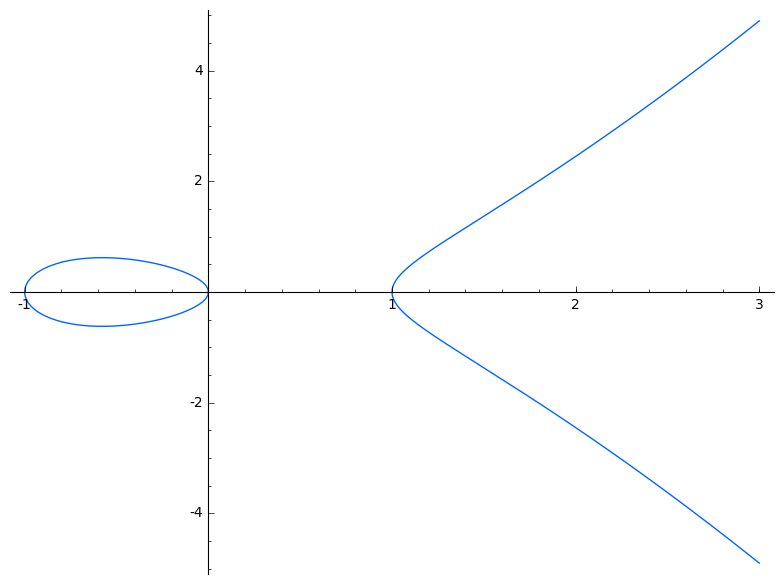
\includegraphics[height=0.5\textwidth, width=0.5\textwidth]{ej1}
    \caption{Salida Código \ref{cod:ej1}}
    \label{fig:ej1}
\end{figure}

Programamos de forma similar el código para visualizar la gráfica de la curva dada por la ecuación $y^2=x^3+x$, véase el Código \ref{cod:ej2}, cuya salida se encuentra en la Figura \ref{fig:ej2}.

\begin{lstlisting}[label={cod:ej2}, caption={Curva elíptica $y^2=x^3+x$}, morekeywords={sage}]
sage: E =  EllipticCurve(RR, [1, 0]);
      plot(E, (-2, 4), color=hue(0.8))
\end{lstlisting}

\begin{figure}[H]
    \centering
    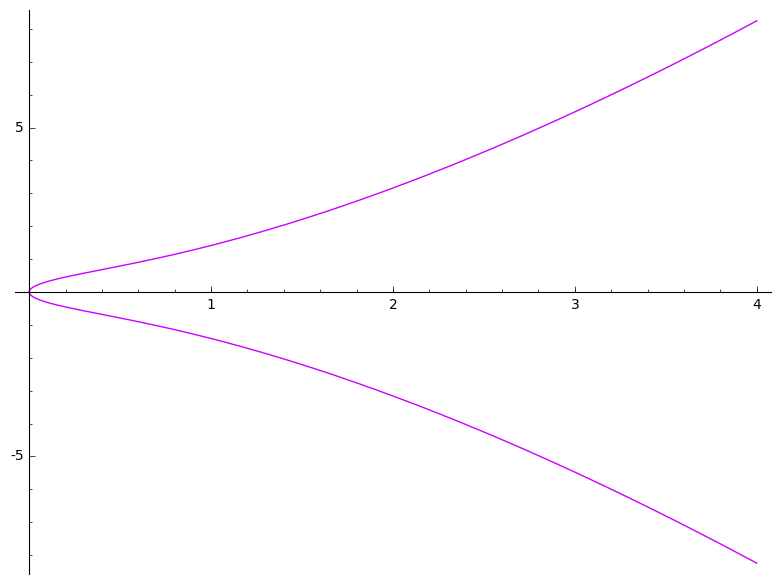
\includegraphics[width=0.5\textwidth]{ej2}
    \caption{Salida Código \ref{cod:ej2}}
    \label{fig:ej2}
\end{figure}

En la Figura \ref{fig:EllipticCurveCatalog} tenemos una tabla con la forma de las curvas elípticas para valores enteros de $a$ entre -2 y 1 y $b$ entre -1 y 2.

\begin{figure}[H]
    \centering
    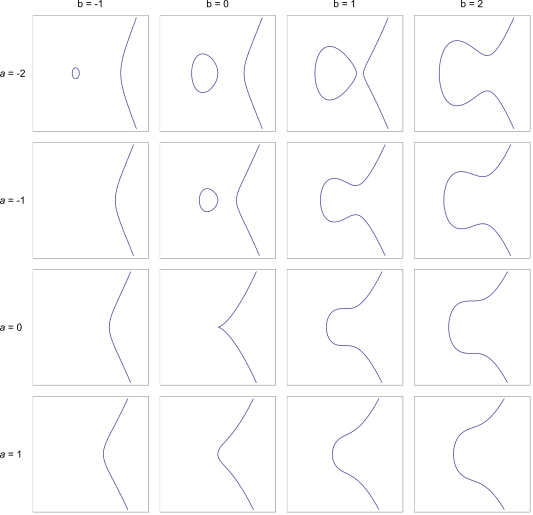
\includegraphics[width=0.7\textwidth]{EllipticCurveCatalog}
    \caption{Ejemplos de curvas elípticas sobre $\mathbb{R}$ (\cite{tos_elliptic_2008})}
    \label{fig:EllipticCurveCatalog}
\end{figure}



\subsection{Estructura de grupo}
Dada una curva elíptica podemos definir un grupo abeliano formado por puntos de la misma. 
\begin{enumerate}
\item Tomamos como elemento neutro el punto del infinito $\infty$.
\item El opuesto de un punto $ P $ viene dado por su simétrico por el eje de abscisas. Más concretamente, si $ P = (x_P, y_P) $ entonces $ -P = (x_P, -y_P) $.
\item En general, dados dos puntos de la curva $ P = (x_P, y_P) $ y $ Q = (x_Q, y_Q) $ con $ x_P \neq x_Q $, su suma es el punto $ -R $ que viene definida por:
\[
(x_R, -y_R) =(m^2 − x_P − x_Q, -y_P - m(x_R − x_P )) = (m^2 − x_P − x_Q, -y_Q - m(x_R − x_Q )),
\]
donde
\[
m = \frac{y_P-y_Q}{x_P-x_Q}.
\]
Definimos $ P+Q=-R $ debido al sentido geométrico de la suma en la curva. Esta operación debe seguir la siguiente regla: ``dados tres puntos $ P$, $ Q $ y $ R $ alineados y no nulos su suma $ P + Q + R $ debe ser el elemento neutro''. Por lo tanto, $ P +Q $ es el opuesto al punto de corte de la recta que une ambos puntos con la curva. De ahí también notamos la presencia del signo menos en la segunda coordenada tal y como indicamos en el punto anterior sobre los opuestos. El sentido geométrico nos aporta intuitivamente la conmutatividad ya que la recta tangente es la misma en el caso $ P+Q $ y $ Q+P $ y la asociatividad ya que $ (P+Q) + R = P + (Q+R) = (P+R) + Q = \infty$.\\

No podemos usar estas fórmulas en algunos casos especiales, por ejemplo cuando $ P=Q $. En este caso no existe una sola recta que pase por ``ambos'' puntos. Sin embargo, si nos aproximamos a $ Q $ mediante puntos $ Q' $ con $ Q' \neq P $ en seguida vemos que la recta que obtendríamos es la tangente en $ P $. Así, definimos su suma como el opuesto del punto de intersección de la recta tangente en $ P $.\\

Otra situación interesante es cuando $ P \neq Q $ pero no hay más puntos de corte. Nos encontramos en un caso parecido al anterior ya que uno de los puntos es tangente a la curva. Si suponemos que $ P $ es donde se da la tangencia, por el caso anterior tememos que $ P + P = -Q $ por lo que $ P + Q = -P $. En estas situaciones de tangencia tenemos que:
\[
m = \frac{3x^{2}_P + a}{2y_P}.
\]
En ambos casos debemos comprobar que la suma pertenece a la curva y que los tres puntos están alineados.

La Figura \ref{fig:EC_add} muestra la idea geométrica de la operación de suma.

\begin{figure}[H]
	\centering
	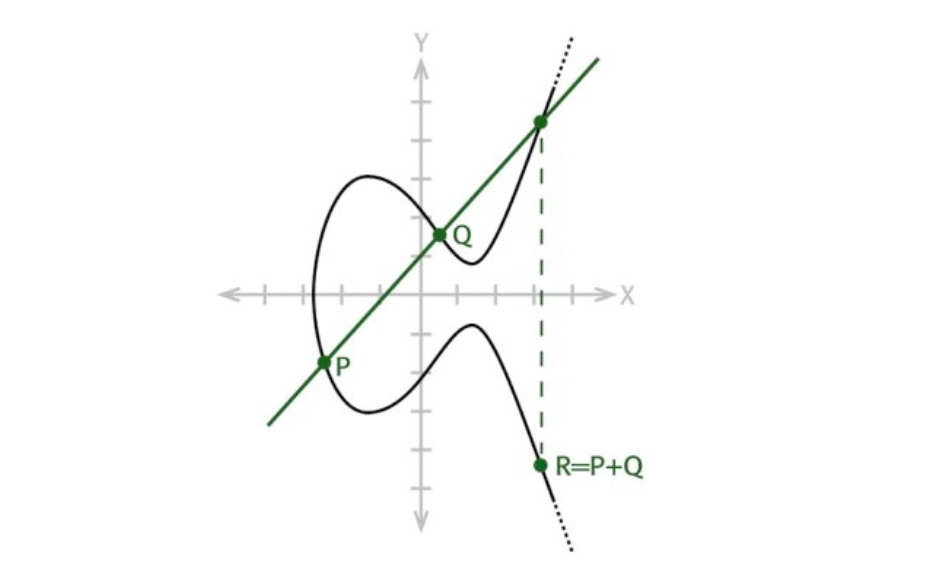
\includegraphics[width=0.7\textwidth]{ec_add}
	\caption{Suma de la curva elíptica $\mathbb{R}$ (\cite{ECC_add})}.
	\label{fig:EC_add}
\end{figure}


\item Finalmente, dado $ n \in \mathbb{Z} $, el producto por escalares lo definimos como:
\[   
nP = 
\begin{cases}
 (P+\stackrel{n}{\cdots}+P) &\text{si } n > 0\\
0 &\text{si } n = 0\\
(-P-\stackrel{n}{\cdots}-P) &\text{si } n < 0\\
\end{cases}.
\]
\end{enumerate}

\subsection{Curvas elípticas sobre cuerpos finitos}
Lo más habitual es que el cuerpo sobre el que trabajemos en criptografía sea un cuerpo finito, $ \mathbb{F}_p $ con $ p $ un primo. En ese caso, la curva vendría dada por:
\[E = \{(x,y) \in K\times K : y^2 \equiv x^3 + ax +b \bmod p,\ 4a^3+27b \not\equiv 0 \bmod p\} \cup \{\infty\}.
\] 

Para ver la representación de las curvas en estos casos ejecutamos el Código \ref{cod:ej5}. Podemos observar el resultado de la ejecución del código con $p=113$ en la Figura \ref{fig:ej5} y para $p=337$ en la Figura \ref{fig:ej6}.

\begin{lstlisting}[language=python, label={cod:ej5}, caption={Curva elíptica $y^2 + y=x^3-x $ sobre $ \mathbb{F}_{p}$.}, morekeywords={sage}]
sage: E = EllipticCurve('37a')
      @interact
      def f(p=primes(2,500)):
          show(plot(E.change_ring(GF(p)),pointsize=30),
               axes=False, frame=True, gridlines="automatic",
               aspect_ratio=1)
\end{lstlisting}

\begin{figure}[H]
	\centering
	\begin{minipage}[b]{0.4\textwidth}
	\centering
	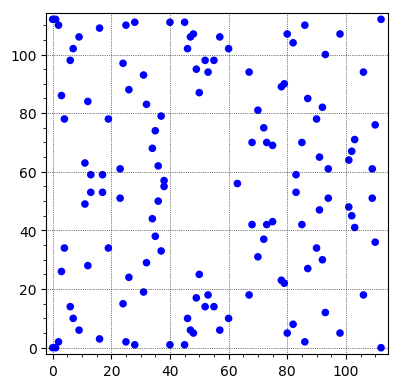
\includegraphics[width=0.6\textwidth]{EC_F_113}
	\caption{Código \ref{cod:ej5} para $ p = 113 $}
	\label{fig:ej5}
	\end{minipage}
	\begin{minipage}[b]{0.4\textwidth}
		\centering
	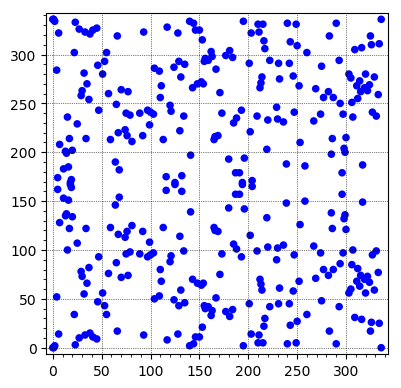
\includegraphics[width=0.6\textwidth]{EC_F_337}
	\caption{Código \ref{cod:ej5} para $ p = 337 $}
	\label{fig:ej6}
	\end{minipage}
\end{figure}

En cuanto a las fórmulas para la operación del grupo, son las mismas que las definidas anteriormente solo que debemos añadir ``$ \mod p $'' a cada una de ellas. Ello conlleva, por ejemplo, la ``repetición'' de la recta que une ambos puntos. La discusión sobre su validez, especialmente en los casos especiales notados anteriormente, requiere de unas matemáticas más profundas en las que no vamos a entrar pero que están estudiadas de manera rigurosa. %TODO añadir referencia que justifique esto


\subsection{Subrupos}
Notamos que si, $ n, m \in \mathbb{Z} $ y $ P \in E $ se cumple que:
\[
nP + mP = (n+m)P.
\]
Así, los múltiplos de $ P $ son cerrados bajo la suma. Obtenemos de este modo que los múltiplos de un punto de la curva forman un subgrupo cíclico. Nos preguntamos ahora cuál es el orden de dichos subgrupos, es decir, debemos encontrar el mínimo $ n \in \mathbb{N} $ que cumpla $ nP = \infty $. Para su cálculo debemos tener en cuenta el Teorema de Lagrange que nos dice que si $ S $ es un subgrupo de $ H $ entonces el orden de $ S $ es un divisor del orden de $ H $. El orden del grupo de la curva elíptica lo podemos calcular en tiempo polinomial gracias al algoritmo de Schoof (\cite{schoof_group_order}). De este modo, como tenemos el orden del grupo formado por la curva elíptica que notamos como $ N $, el orden del subgrupo con generador $ P $ queda determinado por:
\[
\min\{ n \in \mathbb{N}:\text{ } nP = \infty \text{ y } n | N\}.
\]
Normalmente, el proceso seguido en los algoritmos de criptografía de la curva elíptica es el opuesto, es decir, primero elegimos el orden del subgrupo que queremos y posteriormente hallamos el generador. Si el orden del subgrupo es un primo $ p $ el proceso a seguir es el siguiente: calculamos el cofactor $ h = N/n $, tomamos un punto aleatorio $ P \in E $ y obtenemos $ hP $. Si es $\infty$, tomamos un nuevo punto y si no, $ P $ es el generador deseado. Los órdenes de los subgrupos se suelen escoger de orden primo ya que Pohlig y Hellman probaron que un criptosistema es seguro si, y solo si, no es factible el cálculo del logaritmo discreto en grupos con orden un primo (\cite{pohlig1978improved}). En la siguiente sección exponemos el problema del logaritmo discreto en el contexto de las curvas elípticas. \\
%----
\section{El problema del logaritmo discreto}
\label{sec:log}
La seguridad de la criptografía de la curva elíptica reside en la dificultad para calcular logaritmos discretos. Este problema es análogo al de otros criptosistemas como el \textit{Digital Signature Algorithm} (DSA) o el intercambio de claves mediante el mecanismo de Diffie-Hellman.\\

En nuestro caso, el problema consiste en lo siguiente: ``si conocemos $ P $ y $ Q $ dos puntos de la curva elíptica, ?`podemos encontrar un $ k $ tal que $ Q = kP $? ''. Vemos que no estamos calculando un logaritmo como tal pero se sigue usando ese término por analogía a otros sistemas como se ha mencionado anteriormente.\\

Actualmente, no existe ninguna demostración matemática que efectivamente pruebe la dificultad de dicho cálculo. Solo sabemos que es difícil pero no podemos estar seguros. Con el siguiente ejemplo ilustramos su complejidad. Para ello usamos el algoritmo \textit{Baby-step, giant-step} que se basa en el hecho de que cualquier entero $ x $ puede expresar como $ x = am+b $ con $ a,m \text{ y } b$ también enteros. Escribimos entonces:
\begin{equation*}
\begin{split}
Q &= xP \\
  &= (am+b)P\\
  &=amP + bP.
\end{split}
\end{equation*}
Así, podemos expresar $ Q - amP  = bP $. El algoritmo consiste en calcular algunos valores de $ bP $ y otros de $ Q-amP $ hasta que encontremos una correspondencia. El algoritmo también indica que debemos escoger $ m = \sqrt{n} $ y los números $ a $ y $ b $ se mueven entre 0 y $ m $ por lo que mientras $ bP $ tiene incrementos pequeños (\textit{baby}) $ amP $ los tiene grandes (\textit{huge}). Este método nos aporta una complejidad tanto en tiempo como en memoria de $ O(\sqrt{n}) $, es decir, exponencial pero es mejor que uno de fuerza bruta. De todos modos sigue siendo intratable ya que para un $  n  $ tal que $ \sqrt{n} = 7.922816251426434 \times 10^{28} $ el almacenamiento de datos que podemos llegar a necesitar es de $ 2,5\times10^{30} $ bytes de memoria (la capacidad de almacenamiento mundial es de aproximadamente $ 10^{21} $ bytes). \\

\section{Algoritmos}
\label{sec:alg}
Los algoritmos criptográficos basados en curvas elípticas (ECC, por sus siglas en inglés \textit{Elliptic Curve Cryptography}) surgen por primera vez en el año 1984 y muchos de ellos son adaptaciones de algoritmos ya existentes para utilizarlos en el grupo definido por una curva elíptica. En esta sección nos centraremos en dos de esos algoritmos: ECDSA y ECDH, uno de firma y otro de intercambio de claves (\cite{noauthor_elliptic_nodate}).\\

Expuestas todas las herramientas necesarias, falta mencionar cuáles son los parámetros necesarios para los algoritmos. Serán una séxtupla $ (p, a, b, G, n, h) $, donde:
\begin{itemize}
	\item $ p $ es un número primo.
	\item $ a, b $ son los coeficientes de la curva elíptica, hay que elegirlos con cuidado para garantizar que el algoritmo sea seguro.
	\item $ G $ es el generador del subgrupo.
	\item $ n $ es el orden del subgrupo.
	\item $ h $ es el cofactor del subgrupo.
\end{itemize}

En ocasiones también se añade a estos parámetros una semilla que se utiliza mediante una función \textit{hash} para calcular el orden del grupo o los coeficientes de la curva, de esta forma no dependeríamos de la seguridad de una curva específica.\\

La ECC es un tipo de sistema de clave pública, luego es necesario definir cuáles serán las claves utilizadas.

\begin{itemize}
\item La \textbf{clave privada} es un entero aleatorio $d$ elegido en el intervalo $[1,n-1]$.
\item La \textbf{clave pública} es el punto de la curva $H = dG$.
\end{itemize}

Conociendo $d$ y $G$ es fácil encontrar $H$, mientras que conociendo $G$ y $H$ es complejo hallar $d$, como se explicó en la Sección \ref{sec:log}, ya que requiere resolver el problema del logaritmo discreto.


\subsection{ECDH}
ECDH (\textit{Elliptic Curve Diffie Hellman}) es un protocolo para el intercambio de claves basado en Diffie-Hellman. La situación a resolver es la siguiente: Alice y Bob quieren comunicarse de forma privada sin que Carol pueda descifrar sus mensajes. Alice y Bob pueden usar ECDH para generar e intercambiar las claves que les permitan mantener un intercambio de mensajes seguro siguiendo los pasos a continuación:

\begin{enumerate}
\item Comienzan generando sus propias claves. Alice generará su clave privada, $d_A$ y a partir de ella calculará su clave pública $H_A = d_AG$. Bob actuará de la misma forma para obtener sus claves privada, $d_B$, y pública, $H_B = d_BG$. Notamos que los dos deben usar el mismo generador $G$ en la misma curva elíptica definida sobre el mismo cuerpo finito.

\item Alice y Bob intercambian sus claves públicas, $H_A$ y $H_B$, mediante un canal potencialmente inseguro. Carol podría interceptarlas, pero no será capaz de descubrir sus claves privadas sin resolver el problema del logaritmo discreto.\\
\item Para calcular la clave compartida, Alice calcula $C = d_AH_B$ usando su clave privada y la clave pública de Bob. Análogamente, Bob calcula esta clave compartida, será el punto $C = d_BH_A$. Comprobamos que, efectivamente, el punto $C$ es el mismo en ambos casos:
  \[C = d_AH_b = d_A(d_BG) = d_B(d_AG) = d_BH_A = C.\]
\end{enumerate}

Carol, sin embargo, solo conoce $H_A$ y $H_B$ y a partir de estos puntos es incapaz de determinar la clave compartida $C$. Este es el problema de Diffie-Hellman que, en este contexto, se enuncia:
  ``Dados tres puntos $P, aP,$ y $bP$, ¿cuál es el punto resultante de $abP$?''.\\

Se cree que el problema de Diffie-Hellman para curvas elípticas es tan complejo como el problema del logaritmo discreto, aunque no se ha probado.\\

Ahora que Alice y Bob tienen su clave compartida pueden intercambiar mensajes mediante cifrado simétrico, como AES o DES.

\subsection{ECDSA}

ECDSA es un algoritmo de firma digital, \textit{Elliptic Curve Digital Signature Algorithm}, es una variante del algoritmo DSA (\textit{Digital Signature Algortihm}) aplicado a curvas elípticas. Trabaja con el \textit{hash} del mensaje en lugar de con el propio mensaje. La elección de la función \textit{hash} es importante, de esto dependerá la seguridad del sistema criptográfico. El \textit{hash} del mensaje tendrá una longitud de \textit{n} bits\footnote{Si la longitud fuera mayor que $n$, lo truncamos.}, lo denotamos por \textit{z}.\\

Imaginemos que Alice quiere firmar un mensaje con su llave privada, $d_{A}$, y la otra persona, Bob, quiere validar la firma con la clave pública de Alice, $H_{A}$. Alice es la única que puede producir las firmas válidas, sin embargo todo el mundo que tenga su clave pública puede verificarlas.\\

Alice y Bob están usando los mismos parámetros del dominio.

\subsubsection*{Firma del mensaje}
A partir de \textit{k} y \textit{z} se genera la firma con la clave privada de Alice:

\begin{enumerate}
	\item Tomamos un entero $ k $ de forma aleatoria en el conjunto $ \{ 1, ..., n-1\} $.
	\item Calculamos \textit{P} = \textit{kG}.
	\item Hallamos el número \textit{$r \equiv x_{P} \mod n$}.
	\item Si \textit{r} es 0 entonces se toma otro \textit{k} y se intenta de nuevo.
	\item Calculamos $s \equiv k^{-1}(z + rd_{A}) \mod n$  con \textit{$k^{-1}$} el inverso multiplicativo de \textit{k} módulo \textit{n}.
	\item Si \textit{s} es 0 entonces elegimos otro \textit{k} y volvemos al principio.
\end{enumerate} 

Al final obtendremos la firma que será la pareja (\textit{r}, \textit{s}).


\subsubsection*{Verificación de la firma}
Ahora entra en juego Bob que quiere validar la firma, $(r,s)$, a partir del mensaje recibido con valor \textit{hash} \textit{z} y de la clave pública de Alice, $H_A$.

\begin{enumerate}
	\item Calculamos $u_1 \equiv$ \textit{$s^{-1}$ z} mod\textit{n}.
	\item Calculamos $u_2 \equiv$ \textit{$s^{-1}$ r} mod\textit{n}.
	\item Calculamos el punto $P = u_1G + u_2 H_A$.	
\end{enumerate}

La firma solo es válida si $r = x_P \mod n$.
\subsubsection*{Exactitud del algoritmo}
Veamos que esta definición de \textit{P} del punto 3 coincide con la definición original de $P = kG $.

Partimos de \textit{P} = $u_1 G + u_2 H_A$, sustituimos el valor de la clave pública $H_A = d_A G$


\begin{align}
\begin{split}
\textit{P} &= u_1 G + u_2 H_A\\ &= u_1 G + u_2 d_A G\\
&=  (u_1 + u_2 d_A) G.\\
\end{split}
\end{align}

Sustituimos los valores de $u_1$ y $u_2$ que hemos declarado en la verificación de la firma:

\begin{align}
\begin{split}
P &= (u_1 + u_2 d_A) G\\
&= (s^{-1}z + s^{-1} r d_A) G  \\
&= s^{-1}(z + r d_A) G.\\
\end{split}
\end{align}

Como el subgrupo cíclico de orden $n$ en el que estamos trabajando está generado por $G$ no hace falta poner ``$\mod n$'' si multiplicamos por $G$.


Ahora nos fijamos en la definición de $s = k^{-1}(z + r d_A) \mod n$. Multiplicamos por $k$ a ambos lados y dividimos por \textit{s} y obtenemos: $k = s^{-1} (z + r d_A) \mod n$.

\begin{align}
\begin{split}
P &= s^{-1}(z + r d_A) G\\
&= kG.
\end{split}
\end{align}


\subsubsection*{Importancia de $k$}

Es importante el valor que escojamos de \textit{k} el entero aleatorio utilizado para firmar. Si además siempre firmamos con el mismo valor de $k$ y con los mismos valores aleatorios, para los atacantes será más fácil encontrar la clave privada.

Para descubrir la clave privada $d_S$ necesitamos calcular $k$ a partir de los valores \textit{hash} $z_1$ y $z_2$ y de las correspondientes firmas ($r_1$, $s_1$) y ($r_2$, $s_2$).


\begin{enumerate}
	\item $r_1$ es igual a $r_2$, puesto que $ r = x_P \mod n$ y $P = kG$ es el mismo para las dos firmas.
	\item Observamos que  $(s_1 - s_2) \mod n \equiv k^{-1} (z_1 - z_2) \mod n$ viene directamente de la definición de $s$.
	\item $k(s_1 - s_2) \mod n \equiv (z_1 - z_2) \mod n$.
	\item $k  \equiv (z_1 - z_2) (s_1 -s_2)^{-1} \mod n$.
\end{enumerate}

Ahora despejamos $d_S$ de la definición de $s$ y obtenemos que:


\begin{align}
\begin{split}
s &\equiv k^{-1}(z + r d_S) \mod n\\
d_S &\equiv r^{-1}(sk - z) \mod n.\\
\end{split}
\end{align}

Así hemos conseguido la clave privada con los valores que conocemos.

\section{Curvas elípticas más utilizadas}
\label{sec:cur_usa}

Como hemos explicado, los participantes en los algoritmos de cifrado en la curva elíptica deben escoger los mismos parámetros para el dominio. Entre ellos se encuentra la propia curva.\\

Actualmente, existen curvas que son más usadas que otras debido, por ejemplo, al nivel de seguridad que presentan en el cálculo del problema del logaritmo discreto. Destacan:
\begin{enumerate}
\item Spec256k1 (o Curve25519): se utiliza para ECDSA en el modelo criptográfico de Bitcoin (\cite{Secp256k1}). Viene dada por:
\[
y^2 = x^3 + 7.
\]
Se suele utilizar como punto base
\begin{equation*}
\begin{split}
G = (&0\texttt{x}79be667ef9dcbbac55a06295ce870b07029bfcdb2dce28d959f2815b16f81798, \\
		&0\texttt{x}483ada7726a3c4655da4fbfc0e1108a8fd17b448a68554199c47d08ffb10d4b8),
\end{split}
\end{equation*}
que nos aporta un grupo de orden
\[
n =2^{256}-0\texttt{x}14551231950b75fc4402da1732fc9bebf.
\]

\item NIST P-256: es la que trae \textit{OpenSSL} por defecto y he existe una gran cantidad de métodos para optimizar su uso. \\

\item Curve25519: es una de las curvas más rápidas que existen actualmente y su implementación de referencia es de dominio público (\cite{langley_elliptic_nodate}). Viene dada por
\[
y^2 = x^3 + 48662x^2 + x
\]
definida sobre el cuerpo finito con $ 2^{255} - 19 $ elementos el punto base tal que $ x ⁼ 9 $. Esto nos aporta un subgrupo de orden $ 2{^252 }+ 0\texttt{x}14def9dea2f79cd65812631a5cf5d3ed $ (\cite{curve25519}). \\

\item  Curve448: ofrece potencialmente 224 bits de seguridad y aporta un gran rendimiento (\cite{curve448}). Su implementación base está disponible bajo una licencia del MIT. \\
\end{enumerate}
\section{Comparación con RSA}
\label{sec:RSA}
La principal diferencia entre la criptografía de la curva elíptica y la de RSA es el problema en el que basan su seguridad. La curva elíptica lo hace en el problema del logaritmo discreto, mientras que RSA lo hace en el problema de factorización. Otra diferencia fundamental es la cantidad de almacenamiento que se necesita para guardar una clave al mismo nivel de seguridad. Por ejemplo, si para guardar una clave de RSA se necesitan 1024 bits, para almacenar la de ECC se requiere de 160. Las diferencias son aún mayores cuando aumenta el nivel de seguridad, para RSA son necesarios 15360 bits mientras que para ECC tan solo 521 bits.\\ %TODO: referenciar

La relación entre los tamaños no es lineal, es decir, si multiplicamos por \textit{k} el tamaño de RSA, no tenemos \textit{k} veces el tamaño de ECC.

Por otro lado, la generación de la clave y la firma es considerablemente más rápida con ECC que con RSA.

Los algoritmos más rápidos para el cómputo de logaritmos discretos sobre una curva elíptica son Pollard's \textit{rho} y \textit{baby-step giant-step}. Destaca uno en particular que es el algoritmo ``criba general del cuerpo de números'' el más rápido conocido a día de hoy para la factorización de enteros, que además se puede usar para el logaritmo discreto.

%\section{Conclusiones}

\newpage
\printbibliography
\end{document}
